\chapter{Results and Discussion}
\label{chap:05}
\paragraph{}

At last, Runge-Kutta fourth order iteration can be used to optimise and enhance the spring mass model's key parameters and performance. The corresponding relationship between the initial conditions and other parameters of the mass can then be determined. As a result, the spring stiffness of mass and other coefficients can be predicted under different conditions, and the dynamic characteristics can be calculated using the numerical method of Runge-Kutta fourth order method. Therefore, the masses dynamic characteristics are precisely estimated during the masses movemnt processes, and the different processes under various given conditions can be described effectively. The numerical results in this section regarding frequency values and outcomes associated with period and other effective parameters yield the following results for the different spring-mass systems presented in the previous section.

\section{Numerical results for the motion of undamped linear spring mass system with coupled two degrees of freedom}
\paragraph{}

In this section, there are three case studies will discussed with analysis results. Results will be interpreted corresponding to the  different parameter values and initial values. As a result, which helps to identify the precise values of parameters during the experiment. 

\subsection{Case Study 01: Equal initial displacement}
\paragraph{}
 In this subsection, equal initial displacement with different mass values and spring stiffness values will be discussed. The following this method can be used to convert that system into a linear system. To obtain the numerical results earlier stated equations will be used. During this process, mass displacement is the same. Which means $x_1$ and $x_2$ have equal values. And also, with this process, initial velocities ($\Dot{x_1}$ and $\Dot{x_2}$) describe neutral moments, which both have zero values. As given table \ref{tabR1} explains the more details about values of the model's parameters.    
\newpage

 \begin{table}[hbt!]
\begin{center}
    \begin{tabular}{p{6cm}|p{2cm}|p{3cm}}
    \hline
    \textbf{Description of constant} & \textbf{Constant} & \textbf{Values}
    \\
    \hline \hline
    Mass 1 & $m_1$ & 0.815 $(kg)$\\
    Mass 1 & $m_1$ & 3.099 $(kg)$\\
      Spring constant 1  & $k_1$ & 41.5 $(N/m)$\\
      Spring constant 2  & $k_2$  &138 $(N/m)$\\
    Spring constant 3  & $k_3$ & 157.8 $(N/m)$\\
     Initial position of mass 1 & $x_1$ & 0.005 $(m)$ \\
     Initial position of mass 2 & $x_2$ & 0.005 $(m)$  \\
     Initial velocity of mass 1 & $\dot{x_1}$ & 0 $m/s$ \\
     Initial velocity of mass 2 & $\dot{x_2}$ & 0 $m/s$  \\
     Step size & $h$ & 0.1  \\
     Time period & $t$ & 100 $(s)$ \\
     \hline
    \end{tabular}
    \caption{Values of the constant corresponding to the case 01. Values were taken from \cite{JETIRRes28:online}. }
    \label{tabR1}
    \end{center}
\end{table}
  

 \begin{figure}[hbt!]
	\centering
	\begin{framed}
	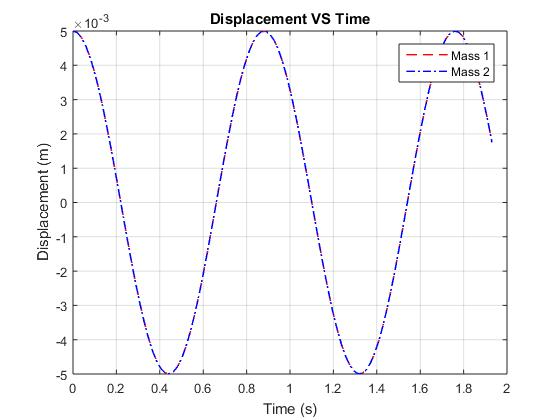
\includegraphics[width=0.7\textwidth]{Figures/R1D.jpg}
		\end{framed}
	\caption{ The displacement of block (mass $m_1$ and mass $m_2$) corresponding to the value from table \ref{tabR1} (case 01).}
	\label{fig:R1}
\end{figure}
 
In this case study 01, equal initial displacement was discussed. As previous stated, in order to analysis this task, initial displacements are 0.005 $m$ both in mass $m_1$ and $m_2$. Figure \ref{fig:R1} depicts the behaviour of displacement over time both masses $m_1$ and $m_2$. Red colour describes the mass 1 ($m_1$) and Blue colour describes the mass 2 ($m_2$). Interestingly, when both masses have same initial displacement which tends to coincide as following figure \ref{fig:R1}. The behaviour of velocity over time both masses $m_1$ and $m_2$ was described in figure \ref{fig:R2}. The velocity curves of the $m_1$ and $m_2$ also tend to coincide with each curve as previous result. 

 \begin{figure}[hbt!]
	\centering
	\begin{framed}
	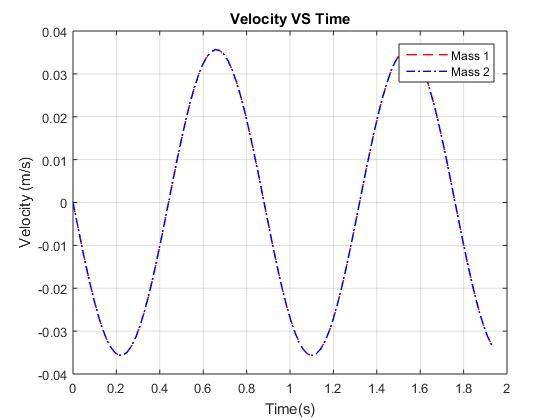
\includegraphics[width=0.7\textwidth]{Figures/R1V.jpg}
		\end{framed}
	\caption{ The velocity of block (mass $m_1$ and mass $m_2$) corresponding to the values from table \ref{tabR1} (case 01).}
	\label{fig:R2}
\end{figure}

\subsection{Case Study 02: Different initial displacement}
\paragraph{}

Now, consider the changing initial conditions and keep the other parameters the same. In this case, only initial displacement of mass 2 ($m_2$) changes into as 0 $m$. Mass 1 ($m_1$) value keeps remain during the process. As earlier used in case 01, in here also initial velocities were kept value as 0 $ms^{-1}$. As a result, figure \ref{fig:R3} was obtained by changing the initial displacement, and this describes the behaviour of the displacement of the $m_1$ and $m_2$. Mass 1 ($m_1$) does have nasty oscillating behaviour during the process, better than mass 2 ($m_2$). Looking at the mass 1 ($m_1$) values, which is less than mass 2 ($m_2$). The smaller amount of $m_1$ displayed a quick, precise behaviour rather than the other mass. When we look at the figure \ref{fig:R4}, the behavior is similar to the behavior discussed in the previous result. The same can be confirmed from the behaviour of mass 1  and mass 2  shown in figure \ref{fig:R4} but it can be observed that they more than oscillated with each other in the previous  velocity described image. Since both masses do not have initial velocities, they both started at zero and ended at the same value. The result we got from this proved to be correct. It can be observed that the eigen frequencies $\omega_1 = 50.9198$ $rads^{-1}$ and $\omega_2 = 264.7758$ $rads^{-1}$ are in this process. Maximum frequency ($f_{max}$) is 2.5898 $Hz$. 



 \begin{figure}[hbt!]
	\centering
	\begin{framed}
	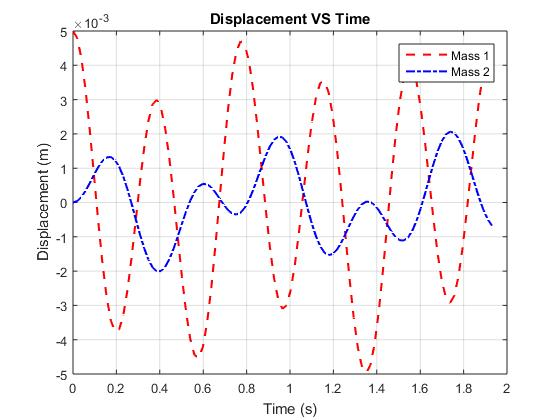
\includegraphics[width=0.7\textwidth]{Figures/R2D.jpg}
	\end{framed}
	\caption{ The displacement of block corresponding to the values from table \ref{tabR1} (case 02). }
	\label{fig:R3}
\end{figure}

\begin{figure}[hbt!]
	\centering
	\begin{framed}
	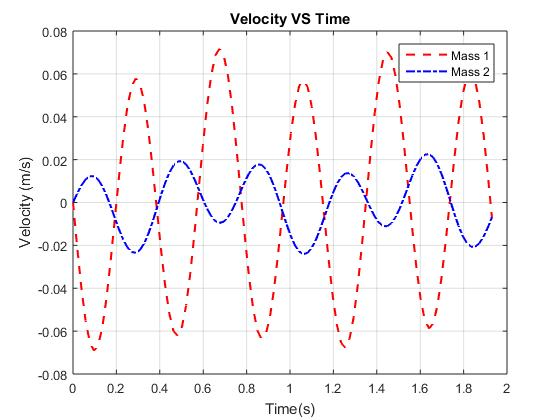
\includegraphics[width=0.7\textwidth]{Figures/R2V.jpg}
		\end{framed}
	\caption{ The velocity of block  corresponding to the values from table \ref{tabR1} (case 02). }
	\label{fig:R4}
\end{figure}

\subsection{Case Study 03: Behavior at the same mass and spring constant values}
\paragraph{}
Now, in order to convert that system into linear system following two method can be implementing. In first case study if
masses having equal initial displacement and, other second case study was change value of $m_2$'s initial displacement. Here, we discuss the interesting case where masses and springs contain the same values.

 \begin{table}[hbt!]
\begin{center}
    \begin{tabular}{p{6cm}|p{2cm}|p{3cm}}
    \hline
    \textbf{Description of constant} & \textbf{Constant} & \textbf{Values}
    \\
    \hline \hline
    Mass 1 & $m_1$ & 0.815 $(kg)$\\
    Mass 1 & $m_1$ & 0.815 $(kg)$\\
    Spring constant 1  & $k_1$ & 41.5 $(N/m)$\\
    Spring constant 2  & $k_2$ & 41.5$(N/m)$\\
    Spring constant 3  & $k_3$ & 41.5 $(N/m)$\\
     Initial position of mass 1 & $x_1$ & 0.005 $(m)$ \\
     Initial position of mass 2 & $x_2$ & 0 $(m)$  \\
     Initial velocity of mass 1 & $\dot{x_1}$ & 0 $m/s$ \\
     Initial velocity of mass 2 & $\dot{x_2}$ & 0 $m/s$  \\
     Time period & $t$ & 100 $(s)$ \\
     \hline
    \end{tabular}
    \caption{Values of the constant corresponding to the case 03. Values were taken from \cite{JETIRRes28:online}. }
    \label{tabR1}
    \end{center}
\end{table}
  
  \begin{figure}[hbt!]
	\centering
	\begin{framed}
	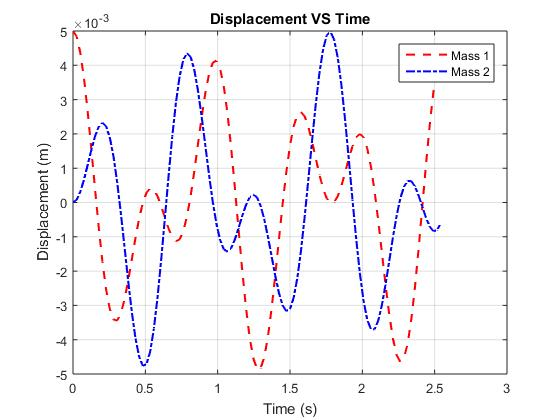
\includegraphics[width=0.7\textwidth]{Figures/R3D.jpg}
		\end{framed}
	\caption{ The displacement of block corresponding to the values from table \ref{tabR1} (case 03). }
	\label{fig:R5}
\end{figure}

  \newpage
  
  
  \begin{figure}[hbt!]
	\centering
	\begin{framed}
	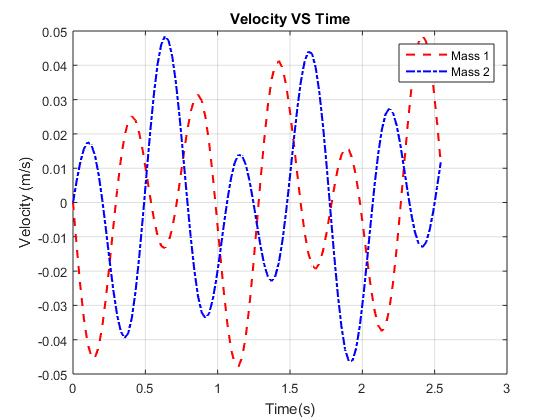
\includegraphics[width=0.7\textwidth]{Figures/R3V.jpg}
		\end{framed}
	\caption{ The velocity of block corresponding to the values from table \ref{tabR1} (case 03). }
	\label{fig:R6}
\end{figure}

When both masses are equal, the obtained expressions are significantly simplified. It can be seen these figure \ref{fig:R5} and figure \ref{fig:R6}. In this case, The mass of the system was set as 0.815 $kg$ in the model.  And the stiffness were set as 41.5 $Nm^{-1}$.  It is interesting to note that the system demonstrates a beating phenomenon, in which energy is transferred cyclically from one mass to the next. It is seen that when the two eigen frequencies are approximately equal. 

\subsection{Summary}
\paragraph{}

 Following table \ref{tbo} explains the details of the each case studies that we have been studied. Looking at the table we realised, the results were obtained by changing a few parameters. 

\begin{table}[h]
\begin{center}
\begin{tabular}{@{}|l|l|l|l|l|l|l|l|l|@{}}
\toprule
Case & $m_1$ $(kg)$ & $m_2$ $(kg)$ & $k_1$ $(N/m)$ & $k_2$ $(N/m)$ & $k_3$ $(N/m)$& $\omega_1$ $(rad/s)$ & $\omega_2$ $(rad/s)$ & $f_{max}$ ($Hz$) \\
\midrule \hline
 1    & 0.815  & 3.099 & 41.5 & 138 & 157.8 & 50.9198 &  264.7758 & 2.5898  \\ 
\hline
2    & 0.815  & 3.099 \footnotemark[1]  & 41.5 & 138 & 157.8 & 50.9198 & 264.7758 & 2.5898 \\ \hline
3    & 0.815  & 0.815  & 41.5 & 41.5 & 41.5 & 50.9202 & 152.7607& 1.9671  \\
\hline
\end{tabular}
\caption{Comparison results}
\label{tbo}
\end{center}
\end{table}

\newpage

\section{Investigate the longitudinal vibrational motion of a (1D) chain}
\paragraph{}
To investigate the dynamics of the vibrational motion in an infinite 1D-chain of identical masses, there are several conditions were considered. To obtain the results, vibration of a linear array of identical atoms corresponding their relevant values will be discussed. In this special case, all the masses are same with its value 0.815 $kg$. And also. in here all the spring constants are same as masses (41.5 $N/m$). The equilibrium separation distance between masses is 0.01 $m$. Using the dispersion relation in above equation discussed in previous section we can calculate their numerical values considering with 100 masses. Following figures will be observed the behaviour of corresponding masses. 


  \begin{figure}[hbt!]
	\centering
	\begin{framed}
	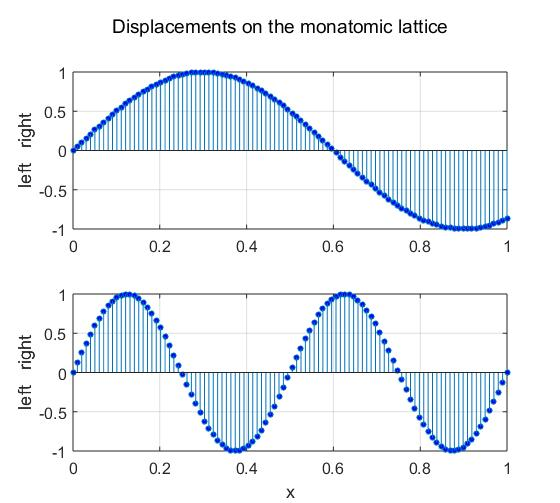
\includegraphics[width=0.8\textwidth]{Figures/N1.jpg}
		\end{framed}
	\caption{ Atomic displacements on the monatomic lattice for a long and short wavelength wave. }
	\label{fig:Lat1}
\end{figure}

Figure \ref{fig:Lat1} shows the results of running the Matlab  with the input parameters: number of masses $n = 100$, separation distance between atoms $d = 0.01$ $m$, mass of each particle $m = 0.815$ $kg$ and spring constant for each spring $k = 10$ $N/m$. In this figure \ref{fig:Lat1} masses displacements on the monatomic lattice for a long and short wavelength wave were displayed. A positive displacement corresponds to a movement to the right and a negative displacement a movement to the left with respect to the equilibrium positions. 

  \begin{figure}[hbt!]
	\centering
	\begin{framed}
	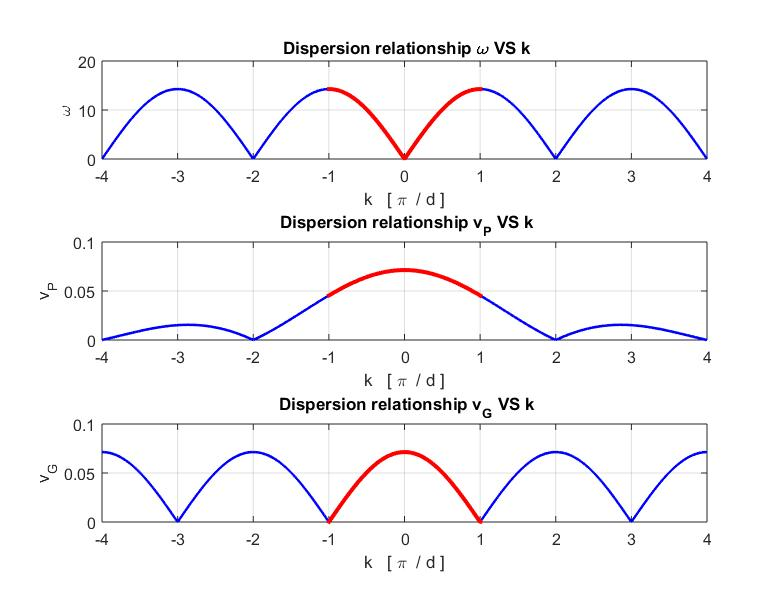
\includegraphics[width=0.9\textwidth]{Figures/N2.jpg}
	\end{framed}
	\caption{ Dispersion relationships for the monatomic lattice. }
	\label{fig:Lat2}
\end{figure}

In this figure \ref{fig:Lat2}, it is seen that particles have been displayed different behaviours due to different conditions. It explains the behaviour of frequency ($\omega$), the behaviour of phase velocity ($V_P$) and the behaviour of group velocity ($V_G$)  with respect to $k_p$. The absolute values must be used, since the frequency is a positive quantity, regardless of whether $k_p$ is positive or negative (which means wave moving to the right or left along the chain). In this process, the maximum angular velocity is $\omega_0$. Above dispersion curve in sub figure 01 clearly shows that for one value of $\omega$ there are several values of wave-vector $k_p$. Therefore we have defined the brillouin zones as first brillouin zone and second brillouin zone. The phase velocity  of a wave is the rate of advance of a point of constant phase along the direction of propagation. In the sub figure 02 explains the phase velocity of the system. A wave is, in general, a superposition of its harmonic components. The ensemble or group of waves is observed to move ahead with a velocity ($d\omega/dt$) known as the group velocity ($V_G$). The group velocity is the velocity with which the wave transmits energy along the propagation direction. No energy can ever be transported past a node in a wave train because the medium at the nodal point is stationary. For the standing waves, the group velocity is zero, and there is zero net energy flow.



\section{Numerical results of two-dimensional spring motion system}
\paragraph{}

This section describes the motion results obtained using Euler's Lagrange equation for a two-dimensional, two-DOF support system comprised of four bilinear springs. The system was obtained by a point mass in a top-view of the four spring mass system, seen in figure \ref{fig:8}. Although, figure \ref{fig:9} depicts the general schematic. As earlier stated, the connector points where one end of every spring connects are considered fixed in space and in line with the two-dimensional plane's $X$ and $Y$ axes. The alignment of the buckles will transform with respect to the original configuration as shown in figure \ref{fig:9} as the mass moves in the two-dimensional plane. These dimensional non linearities will be addressed by calculating the motion's steps at each iteration using Rungre-Kutta fourth order method and updating the equations of motion accordingly. 

\subsection{Case study 01: Behaviour of the mass initial displacement towards the positive $ X $ axis}
\paragraph{}

Case study 01 is defined by the parameters given in
Table 4.1. It is created from the earlier discussed model in section \ref{XY2} and which is only concerned its initial displacement of $X$ axis keeping initial displacement of $Y$ axis zero. 


 \begin{table}[hbt!]
\begin{center}
    \begin{tabular}{p{6cm}|p{2cm}|p{3cm}}
    \hline
    \textbf{Description of constant} & \textbf{Constant} & \textbf{Values}
    \\
    \hline \hline
    Mass of particle  & $m$ & 0.815 $(kg)$\\
      Spring constant of particle  & $k$ & 41.5 $(N/m)$\\
     Initial position of mass $X$ axis & $x$ & 0.005 $(m)$ \\
     Initial position of mass $Y$ axis  & $y$ & 0 $(m)$  \\
     Initial position of mass $X$ axis & $\dot{x}$ & 0 ($m/s$) \\
     Initial position of mass $Y$ axis & $\dot{y}$ & 0 ($m/s$)  \\
     Length of the spring & $l$ & 0.01 ($m$) \\
     Step size & $h$ & 0.01  \\
     Time period & $t$ & 100 $(s)$ \\
     \hline
    \end{tabular}
    \caption{Values of the constant corresponding to the  2D case 01. Mass is moving in $XY$ plane. Several values were taken from \cite{JETIRRes28:online}. }
    \label{tab2D1}
    \end{center}
\end{table}

\newpage 

 \begin{figure}[hbt!]
	\centering
	\begin{framed}
	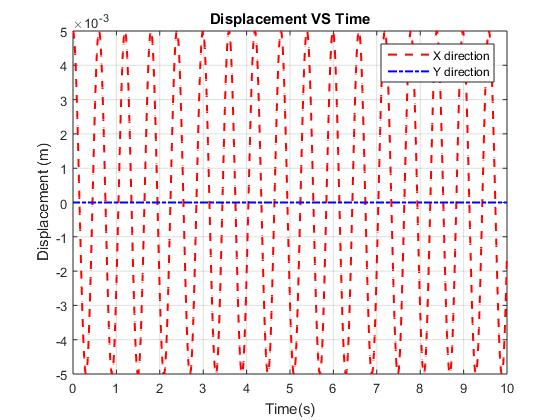
\includegraphics[width=0.66\textwidth]{Figures/2DD.jpg}
		\end{framed}
	\caption{ The displacement of block corresponding to the values from table \ref{tab2D1} (case 01). }
	\label{fig:R5}
\end{figure}

 \begin{figure}[hbt!]
	\centering
	\begin{framed}
	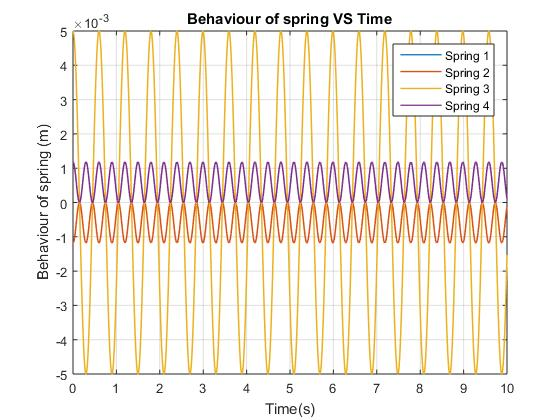
\includegraphics[width=0.66\textwidth]{Figures/2DA.jpg}
	\end{framed}
	\caption{ The displacement of all springs corresponding to the values from table \ref{tab2D1} (case 01). }
	\label{fig:R5}
\end{figure}

 \begin{figure}[hbt!]
	\centering
	\begin{framed}
	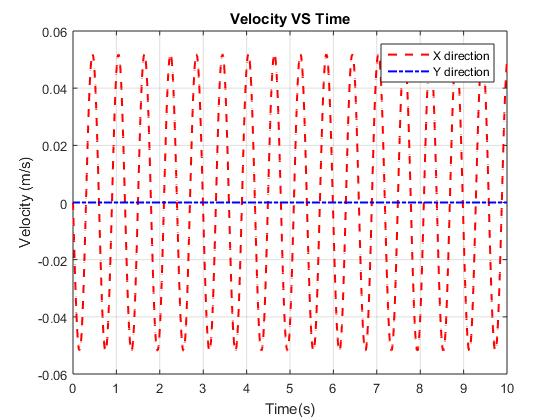
\includegraphics[width=0.7\textwidth]{Figures/2DV.jpg}
		\end{framed}
	\caption{ The velocity of block (mass $m$) corresponding to the values from table \ref{tab2D1} (case 01). }
	\label{fig:R5}
\end{figure}

\newpage

\subsection{Case 02:  Behaviour of the mass initial displacement towards the both positive $X$ and $Y$ axis }
\paragraph{}

In this scenario, Mass has different initial displacements towards both $X$ and $Y$ axis. In the previous case, which has only positive initial displacement  towards $X$  direction. It was set as 0.01 $m$. %To obtain the results, towards $X$ axis displacement and $Y$ axis displacement were assigned as 0.005 $m$ respectively.   

 \begin{table}[hbt!]
\begin{center}
    \begin{tabular}{p{6cm}|p{2cm}|p{3cm}}
    \hline
    \textbf{Description of constant} & \textbf{Constant} & \textbf{Values}
    \\
    \hline \hline
    Mass of particle  & $m$ & 0.815 $(kg)$\\
      Spring constant of particle  & $k$ & 41.5 $(N/m)$\\
     Initial position of mass $X$ axis & $x$ & 0.005 $(m)$ \\
     Initial position of mass $Y$ axis  & $y$ & 0.03 $(m)$  \\
     Initial position of mass $X$ axis & $\dot{x}$ & 0 ($m/s$) \\
     Initial position of mass $Y$ axis & $\dot{y}$ & 0 ($m/s$)  \\
     Length of the spring & $l$ & 0.01 ($m$) \\
     Step size & $h$ & 0.01  \\
     Time period & $t$ & 100 $(s)$ \\
     \hline
    \end{tabular}
    \caption{Values of the constant corresponding to the  2D case 02. Mass is moving in $XY$ plane. Several values were taken from \cite{JETIRRes28:online}. }
    \label{tab2D2}
    \end{center}
\end{table}

\newpage

 \begin{figure}[hbt!]
	\centering
	\begin{framed}
	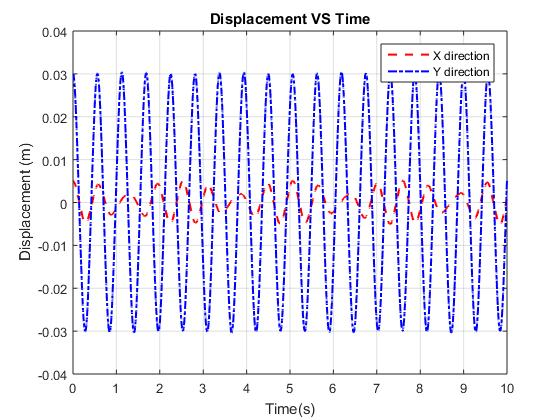
\includegraphics[width=0.66\textwidth]{Figures/2DD2.jpg}
		\end{framed}
	\caption{ The displacement of block corresponding to the values from table \ref{tab2D2} (case 02). }
	\label{fig:221}
\end{figure}

 \begin{figure}[hbt!]
	\centering
	\begin{framed}
	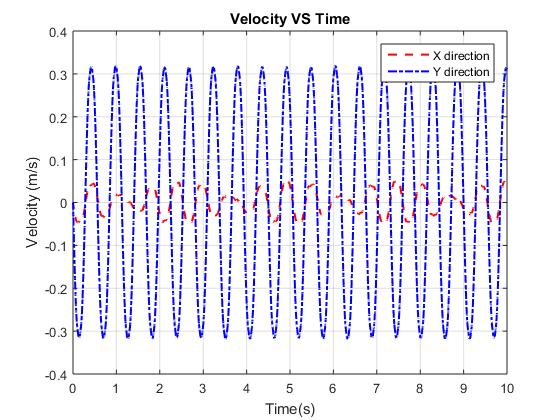
\includegraphics[width=0.66\textwidth]{Figures/2DV2.jpg}
	\end{framed}
	\caption{ The velocity of block corresponding to the values from table \ref{tab2D2} (case 02). }
	\label{fig:222}
\end{figure}

\newpage


 \begin{figure}[hbt!]
	\centering
	\begin{framed}
	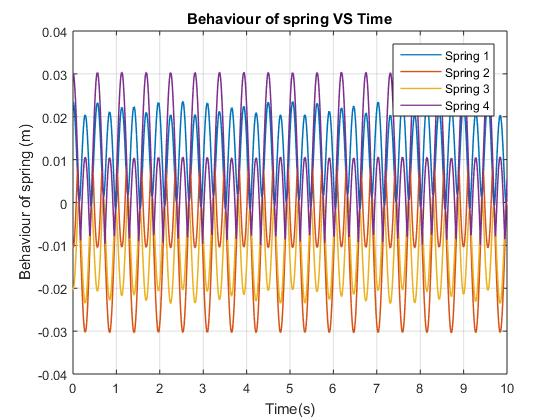
\includegraphics[width=0.7\textwidth]{Figures/2DA2.jpg}
		\end{framed}
	\caption{ The displacement of all springs together corresponding to the values from table \ref{tab2D1} (case 02). }
	\label{fig:223}
\end{figure}

Corresponding to the table \ref{tab2D2} the above results were observed. As shown in figure \ref{fig:221} it can be seen that the displacement of  mass along both $X$ and $Y$ directions. As shown in table  \ref{tab2D2} initial conditions of $x$ and $y$ were defined as 0.005 $m$ and 0.03 $m$ respectively. $y$ has a bigger value than $x$ value. It occurs graphical quality lines corresponding to the given $y$ value. Figure \ref{fig:222} shows the velocity of  mass along both $X$ and $Y$ directions and which depicts the same result that earlier discussed. 

\subsection{Case study 03: Isotropic oscillations 
}
\paragraph{}

In this section, Isotropic oscillations of mass $m$ moving in the two-dimensional will be discussed. To obtain the results, equations \eqref{f1} and \eqref{f2} from section \ref{xo} will be used. In this results phase difference ($\Delta$) will play a major role. The real data of the system are shown in table.  The experimental analysis for the movement of the mass system was done with given values.  

\begin{table}[h]
\begin{center}

\begin{tabular}{@{}|l|l|l|l|l|l|l|l|@{}}
\toprule
 $m$ $(kg)$  & $k$ $(N/m)$ & $l$ $(m)$ & $\omega$ $(rad/s)$& $T (s)$ & $A$ & $B$  & $\Delta$ \\
\midrule \hline
 0.815    & 41.5  & 0.01 & 10.30 & 0.61&  1 &  1& $ 0, \pi/4, \pi/2, 3\pi/4  $  \\ 
\hline
\end{tabular}
\caption{Real data of the system \cite{JETIRRes28:online,levitan1960forced}}
\label{phase1}%
\end{center}
\end{table}

\newpage


 \begin{figure}[hbt!]
	\centering
	\begin{framed}
	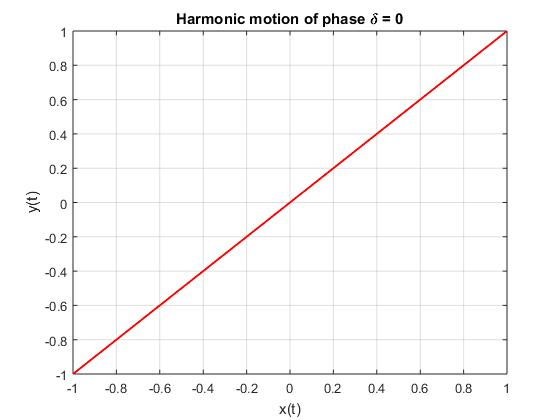
\includegraphics[width=0.68\textwidth]{Figures/0.jpg}
	\end{framed}
	\caption{ Trajectories in a two-dimensional harmonic oscillator potential when $\Delta = 0$. }
	\label{fig:O1}
\end{figure}

 \begin{figure}[hbt!]
	\centering
	\begin{framed}
	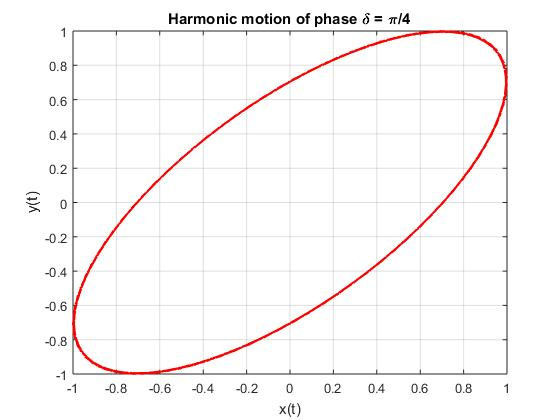
\includegraphics[width=0.68\textwidth]{Figures/p4.jpg}
		\end{framed}
	\caption{ Trajectories in a two-dimensional harmonic oscillator potential when $\Delta = \pi/4 $. }
	\label{fig:O2}
\end{figure}

\newpage

 \begin{figure}[hbt!]
	\centering
	\begin{framed}
	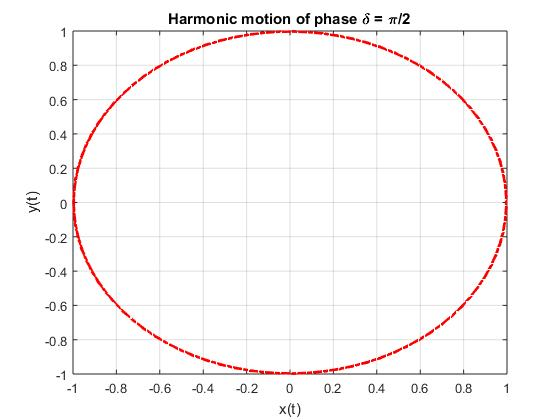
\includegraphics[width=0.68\textwidth]{Figures/p2.jpg}
		\end{framed}
	\caption{ Trajectories in a two-dimensional harmonic oscillator  when $\Delta = \pi/2 $.). }
	\label{fig:03}
\end{figure}


 \begin{figure}[hbt!]
	\centering
	\begin{framed}
	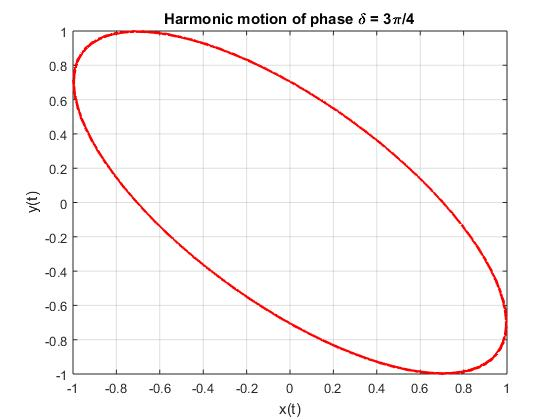
\includegraphics[width=0.68\textwidth]{Figures/3p.jpg}
	\end{framed}
	\caption{ Trajectories in a two-dimensional harmonic oscillator  when $\Delta = 3\pi/4 $. }
	\label{fig:04}
\end{figure}

\newpage

Thus, the combined motion of two simple-harmonics oscillators, one along each axis, with the same angular frequency but differing amplitudes and phase angles, will ensue. The above results prove that they will differ according to their relevant phase difference. Two-dimensional motion of a simple-harmonic oscillator with $A=B=1 m$ and $\Delta= 0$ is shown in figure \ref{fig:O1}. When $\Delta = 0$, the elliptical path of a two-dimensional isotropic oscillator illustrated as shown in figure \ref{fig:O2}. In particular, if the phase difference is equal to $\pi/2$ and $3\pi/4$ in respectively, the results were displayed as shown in figure \ref{fig:03} and  figure \ref{fig:04}. 

\subsection{Case study 04: Anisotropic oscillations}
\paragraph{}
The dynamics of a mass coupled springs are depicted by the  anisotropic oscillator model. In this section, anisotropic oscillations the combined motion of two simple-harmonics oscillators and trajectory map  will be discussed. In this process, both angular frequencies are not same during the process. But other initial conditions keep remain as discussed in table \ref{phase1}. Further, results will be observed two different situations of angular frequencies. The cases can be described as $\omega_x = 2\omega_y$ and $\omega_x = \sqrt{2}\omega_y$.  


 \begin{figure}[hbt!]
	\centering
	\begin{framed}
	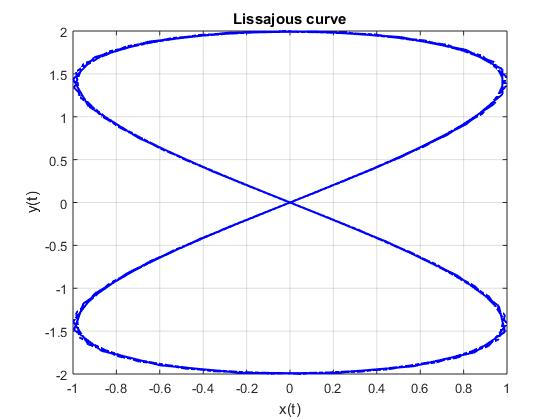
\includegraphics[width=0.7\textwidth]{Figures/Lissajous curve.jpg}
	\end{framed}
	\caption{ Anisotropic oscillations when $\omega_x = 2\omega_y$. }
	\label{fig:O5}
\end{figure}

\newpage

 \begin{figure}[hbt!]
	\centering
	\begin{framed}
	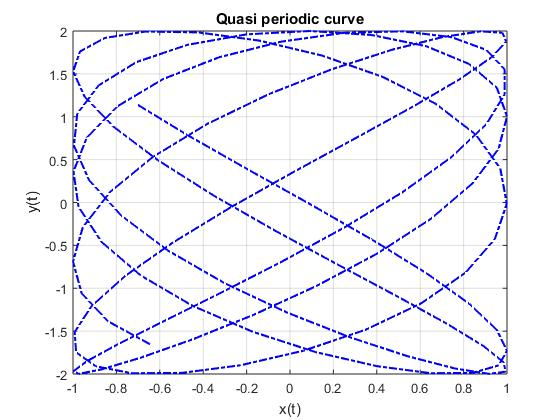
\includegraphics[width=0.7\textwidth]{Figures/quasi periodic.jpg}
	\end{framed}
	\caption{ Quasi periodic curve when $\omega_x = \sqrt{2}\omega_y$. }
	\label{fig:O6}
\end{figure}

The above results were obtained corresponding to the different angular frequencies ($\omega_x \neq \omega_y$). The first result, figure \ref{fig:O5} displayed motion of particle hen $\omega_x = 2\omega_y$. They differ in general, and their ratio determines the mass's orbit in 2-D space. The motion of the mass creates a Lissajous figure is as shown in \ref{fig:O5}.